\documentclass[man, noapacite]{apa2}

\usepackage{url}
% \usepackage{pslatex}
\usepackage{pdfsync}
\usepackage{apacite2}
\usepackage{amsmath}
\usepackage{graphicx}
\usepackage{topcapt}
\usepackage{color}

\title{Negation is only hard to process when it is pragmatically uninformative}
% \title{Processing difficulty of negation is predicted by speakers' likelihood of using negation in context}
\author{Ann E. Nordmeyer and Michael C. Frank}
\affiliation{Department of Psychology, Stanford University}

\shorttitle{Pragmatics of negation}

\abstract{Negation is a fundamental element of language and logical systems, but processing negative sentences can be challenging. Previous work suggests that a supportive context can mitigate the processing costs of negation.  We investigate the role of context on negative sentences by measuring the processing cost of negation in different contexts.  We find that a supportive visual context has a graded effect on negation processing.  Reaction times to respond to both positive and negative sentences were predicted by participants' descriptions of the same stimuli.  Our data suggest that in the right context, representing negation may be less difficult than previously supposed.}  

\acknowledgements{This material is based upon work supported by the National Science Foundation Graduate Research Fellowship. }

\begin{document}
\maketitle

%%%%%%%%% INTRO %%%%%%%%% 
\section{Introduction}

Language is a powerful tool that allows us to describe not only the state of the world as we see it, but also the world as it is not. Nevertheless, for human language users, processing negation is often slow and effortful. Deciding the truth value of a sentence like ``star isn't above plus'' takes a lot longer than making the same decision about a positive sentence \cite{hclark1972, carpenter1975, just1971, just1976}. And in language comprehension tasks as well, participants often show evidence consistent with having processed the positive components of a sentence prior to negating them, suggesting again that negation is slow \cite{kaup2003, kaup2006, hasson2006, fischler1983, ludtke2008}. 

Yet not all negations are equally felicitous. For example, it would be strange for a barista to greet a customer by saying ``we don't have any chai''---unless he was talking to a regular who always ordered chai. And it would be even weirder if he then said ``we don't have any carburetors.'' On Gricean and neo-Gricean accounts of the pragmatics of language use in context, listeners expect speakers to produce informative and relevant utterances \cite{grice1975, horn1984, levinson2000}. The caf\'e's lack of chai would be less informative if the customer didn't want chai, and the subsequent remark about carburetors is both uninformative \emph{and} irrelevant. But is this kind of pragmatic infelicity generally responsible for the processing cost of negation?

Consistent with this suggestion, presenting negative information in a supportive context can mitigate some of its processing costs \cite{wason1965, glenberg1999}. Contexts that explicitly mention a negated characteristic \cite{ludtke2006} or that present negation within a dialogue \cite{dale2011} tend especially to be processed faster.  And in an ERP experiment, contextually-supported negations (e.g., ``with proper equipment, scuba-diving isn't very dangerous'') elicited smaller N400 responses---a marker of semantic processing costs---than unlicensed negations \cite<e.g., ``bulletproof vests aren't very dangerous''>{nieuwland2008}.

Although this previous work supports the idea that some kind of contextual expectations are the source of negation's processing cost, they do not specify the precise nature of these expectations. Drawing on a recent theoretical model of pragmatic reasoning \cite{frank2012}, we define pragmatic expectations in context as the probability that a speaker would utter a statement in order to convey a particular meaning. Our current experiment directly test two hypotheses. First, expectations about what speakers would likely say---and their match or mismatch with what the speaker in fact \emph{does} say---are responsible for the processing costs of negation. Second, RELEVANCE AND INFORMATIVENESS.

In our experiment, we show participants sets of characters who are identical except for the presence or absence of a feature (e.g., boys with or without apples). In the \emph{speaker} condition, we ask participants to produce written descriptions that pick a particular target character out of the set; while in the \emph{listener} condition, we ask participants to evaluate the truth value of negative or positive statements about the target character. Our predictions are: A) that the processing cost for listeners of a negative sentence for a target should be predicted by the surprisal \cite{levy2008} related to a speaker using negation to describe that target. B) that...

\section{Method}

\subsection{Participants} 

%NOTE: These ns are correct & checked
We recruited 489 participants (262 male and 224 female, three declined to report gender; ages 18 -- 65+) to participate in an online experiment through the Amazon's Mechanical Turk (mTurk) website.  We restricted participation to individuals in the US and paid 50 cents for this 10 minute study.  Participants were randomly assigned to either the speaker condition (n = 296) or the listener condition (n = 193).

\subsection{Stimuli}

\begin{figure}[t]
\begin{center} 
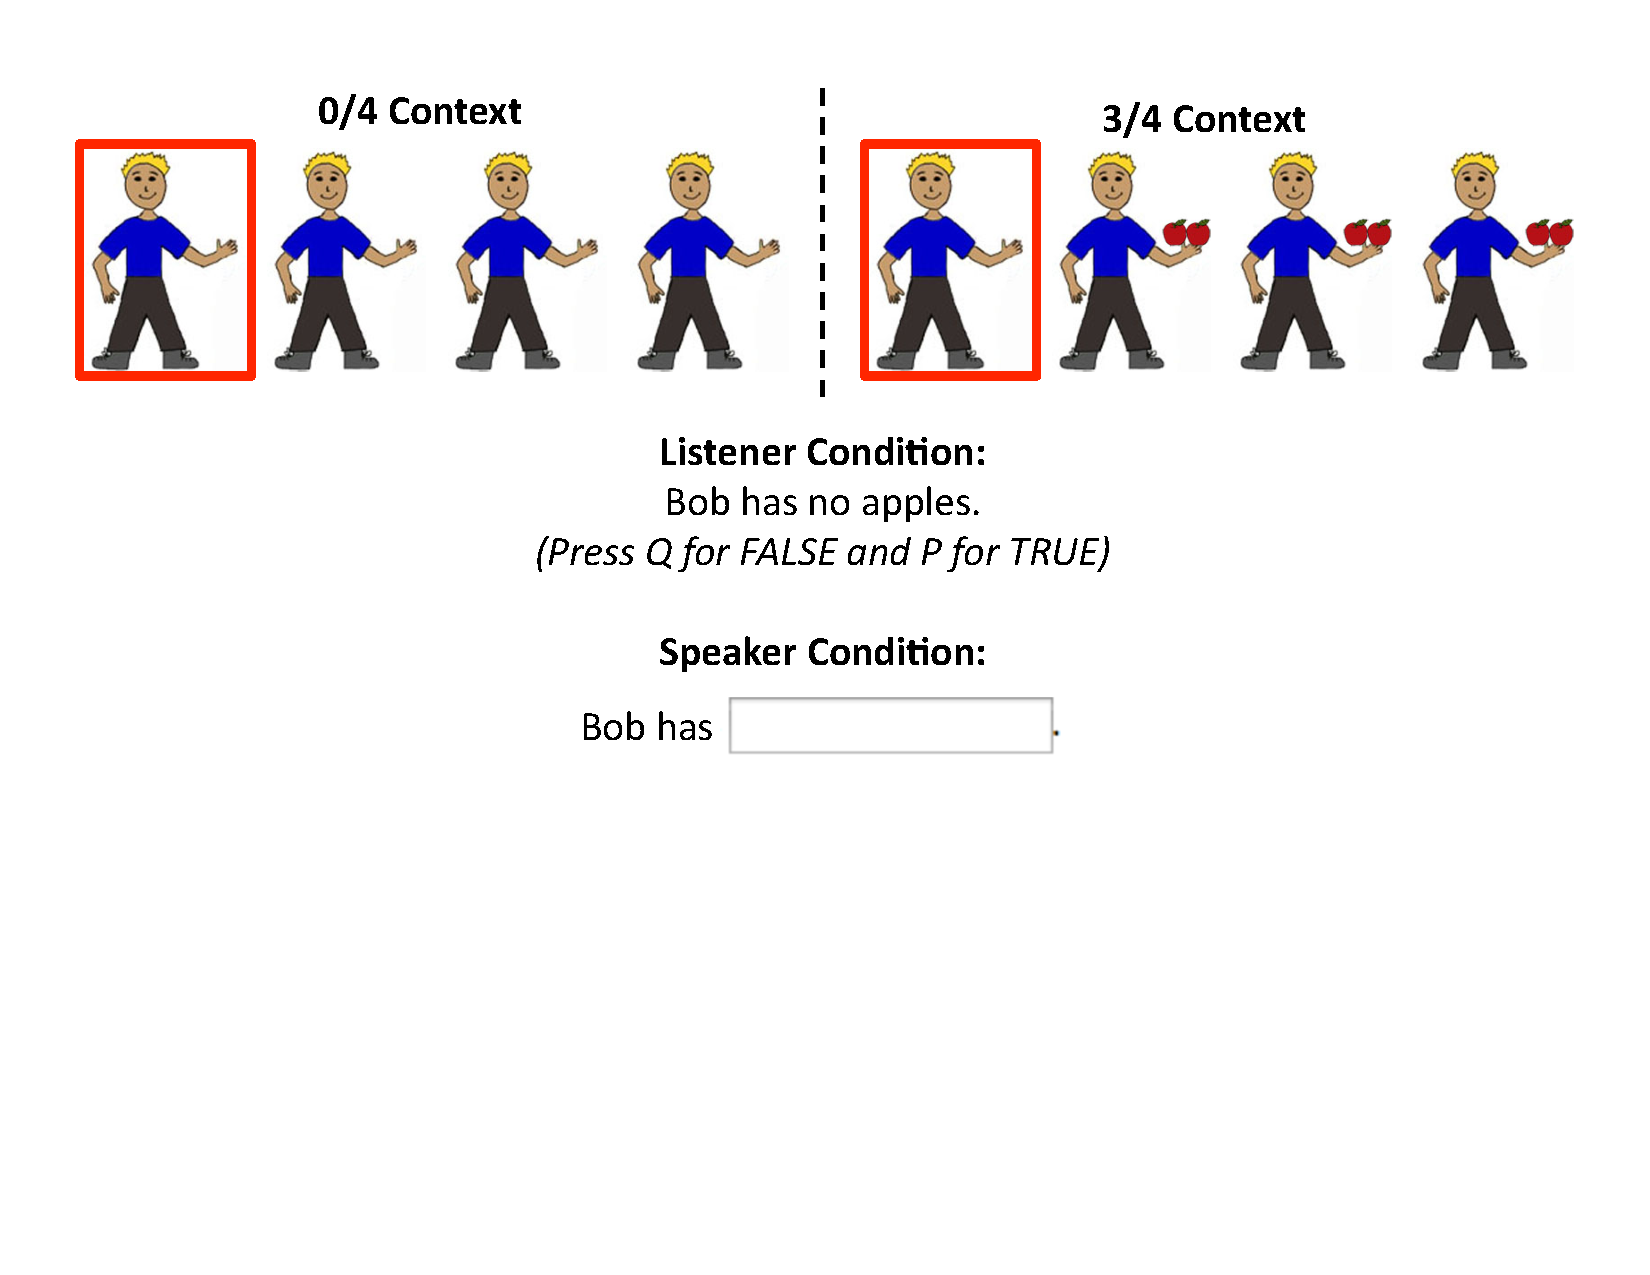
\includegraphics[width=4in]{figures/trialfig.pdf}
\caption{\label{fig:trial} An example of a true negative trial with a 3/4 context. \textcolor{blue}{Modify figure to show what text the two conditions saw, rather than putting in comment text?}}
\vspace{-5mm}
\end{center} 
\end{figure}

Thirty-two trial items were created in which characters were shown holding either two of the same common, recognizable objects (``target items'', e.g. two apples), or holding nothing.  Within each trial, all characters were identical except for the presence or absence of objects; characters varied in appearance (e.g. skin tone, hair color, clothing, gender) across trials.\footnote{Our previous work indicates that the results reported here are robust to a number of changes to the stimuli, including whether the context characters varied in appearance or not.  Results from these previous experiments can be seen in \citeA{nordmeyer2014}.}

A within-subjects factor determined what type of context participants saw on each trial.  The context condition determined the proportion of characters who were holding target items.  Context conditions showed $\frac{0}{4}$, $\frac{1}{4}$, $\frac{2}{4}$, $\frac{3}{4}$, or $\frac{4}{4}$ of the characters holding objects. The order of characters was shuffled on each trial, with the referent of the sentence appearing in a random position.  

\subsubsection{Listener Condition}
For participants in the listener condition, on each trial a sentence of the form ``[NAME] [has/has no] [ITEM]'' appeared.  Half of the sentences were positive and half were negative, and they were paired with pictures such that half were true and half were false.  The experiment was fully crossed, with participants receiving eight true positive, eight false positive, eight true negative and eight false negative sentences distributed equally across context types in a randomized order over the course of the study.  

\subsubsection{Speaker Condition}
Participants in the speaker condition saw the same images paired with an incomplete sentence (e.g. ``[NAME] has $\rule{3cm}{0.15mm}$.''). In half of the trials, the highlighted picture was holding target items, and in half of the trials, the highlighted picture was holding nothing.  The experiment was fully crossed such that target characters appeared with or without target items an equal number of times in each context type.  

\subsection{Procedure}
Participants were first presented with a brief overview screen which explained that they would play a language game.  Once participants accepted the task, they were randomly assigned to either the listener condition or the speaker condition, and saw a more detailed instructions screen which explained the task and informed them that they could stop at any time.  

\subsubsection{Listener Condition}

In the listener condition, participants first saw eight positive sentence practice trials with feedback about incorrect responses before beginning the test trials. 

In each test trial, participants saw an array of four pictures presented in a randomized order.  Participants were told to look at these pictures for four seconds, at which point a red box appeared around one of the pictures.  One second later, a sentence about that picture appeared.  Participants were told to read the sentence and respond as quickly and accurately as possible with a judgment of whether it was true or false when applied to the highlighted picture.  We recorded reaction times for each trial, measured as the time from when the sentence was presented to the moment when the response was made.\footnote{The listener condition of the experiment can be viewed at 
FIXME (I can't get the link to work, it is clickable but sends to the wrong place due to the line break??) \url{https://langcog.stanford.edu/expts/AEN/negatron_production2/negatron.html}.}

\subsubsection{Speaker Condition}

In each trial, participants saw an array of four pictures: The target pictures and three context pictures presented in a random order.  Participants were told to look at these pictures for four seconds, at which point a red box appeared around one of the pictures.  One second later, an incomplete sentence appeared.  Participants were told to finish the sentence (by typing into a small text box) using only a few words, in a way that would help someone else identify the character in the red box if they saw the pictures in a different order.\footnote{The listener condition of the experiment can be viewed at 
FIXME (I can't get the link to work, it is clickable but sends to the wrong place due to the line break??) \url{https://langcog.stanford.edu/expts/AEN/negatronv20/negatron.html}.}
  

 
 \subsection{Data Processing} 
  
We excluded 18 participants who did not list English as their native language and two participants from the listener condition for having an overall accuracy below 80\%, leaving a total of 469 participants for analysis (186 in listener condition, 283 in speaker condition). 

\subsubsection{Listener Condition}
We excluded trials with RTs greater than 3 standard deviations from the log-transformed mean.  

\subsubsection{Speaker Condition}
Affirmative responses labeling the target feature were coded as ``positive'' (e.g. ``apples'', ``two apples'', ``red apples'', etc.).  Responses with a negative element (``no'', ``not'', ``nothing'', ``empty'', or ``zero'') were coded as ``negative''.  All other responses (e.g. descriptions of the characters' clothing or hair color) were coded as ``other''.  Codes were hand-checked to ensure that label synonyms or spelling errors were coded correctly.  

Due to the Gricean nature of the intuition---which lead us to consider a truthful speaker as well---we focused on predicting the processing of true or correct sentences.   We calculated the proportion of positive sentences describing characters who possessed target items, and the proportion of negative sentences describing characters with nothing, creating a probability distribution for true positive and true negative utterances.  We then used this to calculate the surprisal (an information-theoretic measure of the amount of information carried by an event; see \cite{levy2008}) of a positive or negative sentence for each trial type.  

\begin{equation}\label{eq:surprise}
Surprisal = -\log(P(sentence)).
\end{equation}

%NOTE: We should talk about the best way to present the speaker data.  What I've done here is pretty sparse (I really just jump right to surprisal, describing how we calculate that here and then describing the relationship between surprisal and RT in the results section.  I'm wondering if we should present a table of the probabilities in response to each trial type, though?)

\section{Results}

\subsection{Listener Condition}

\begin{figure}[t]
\begin{center} 
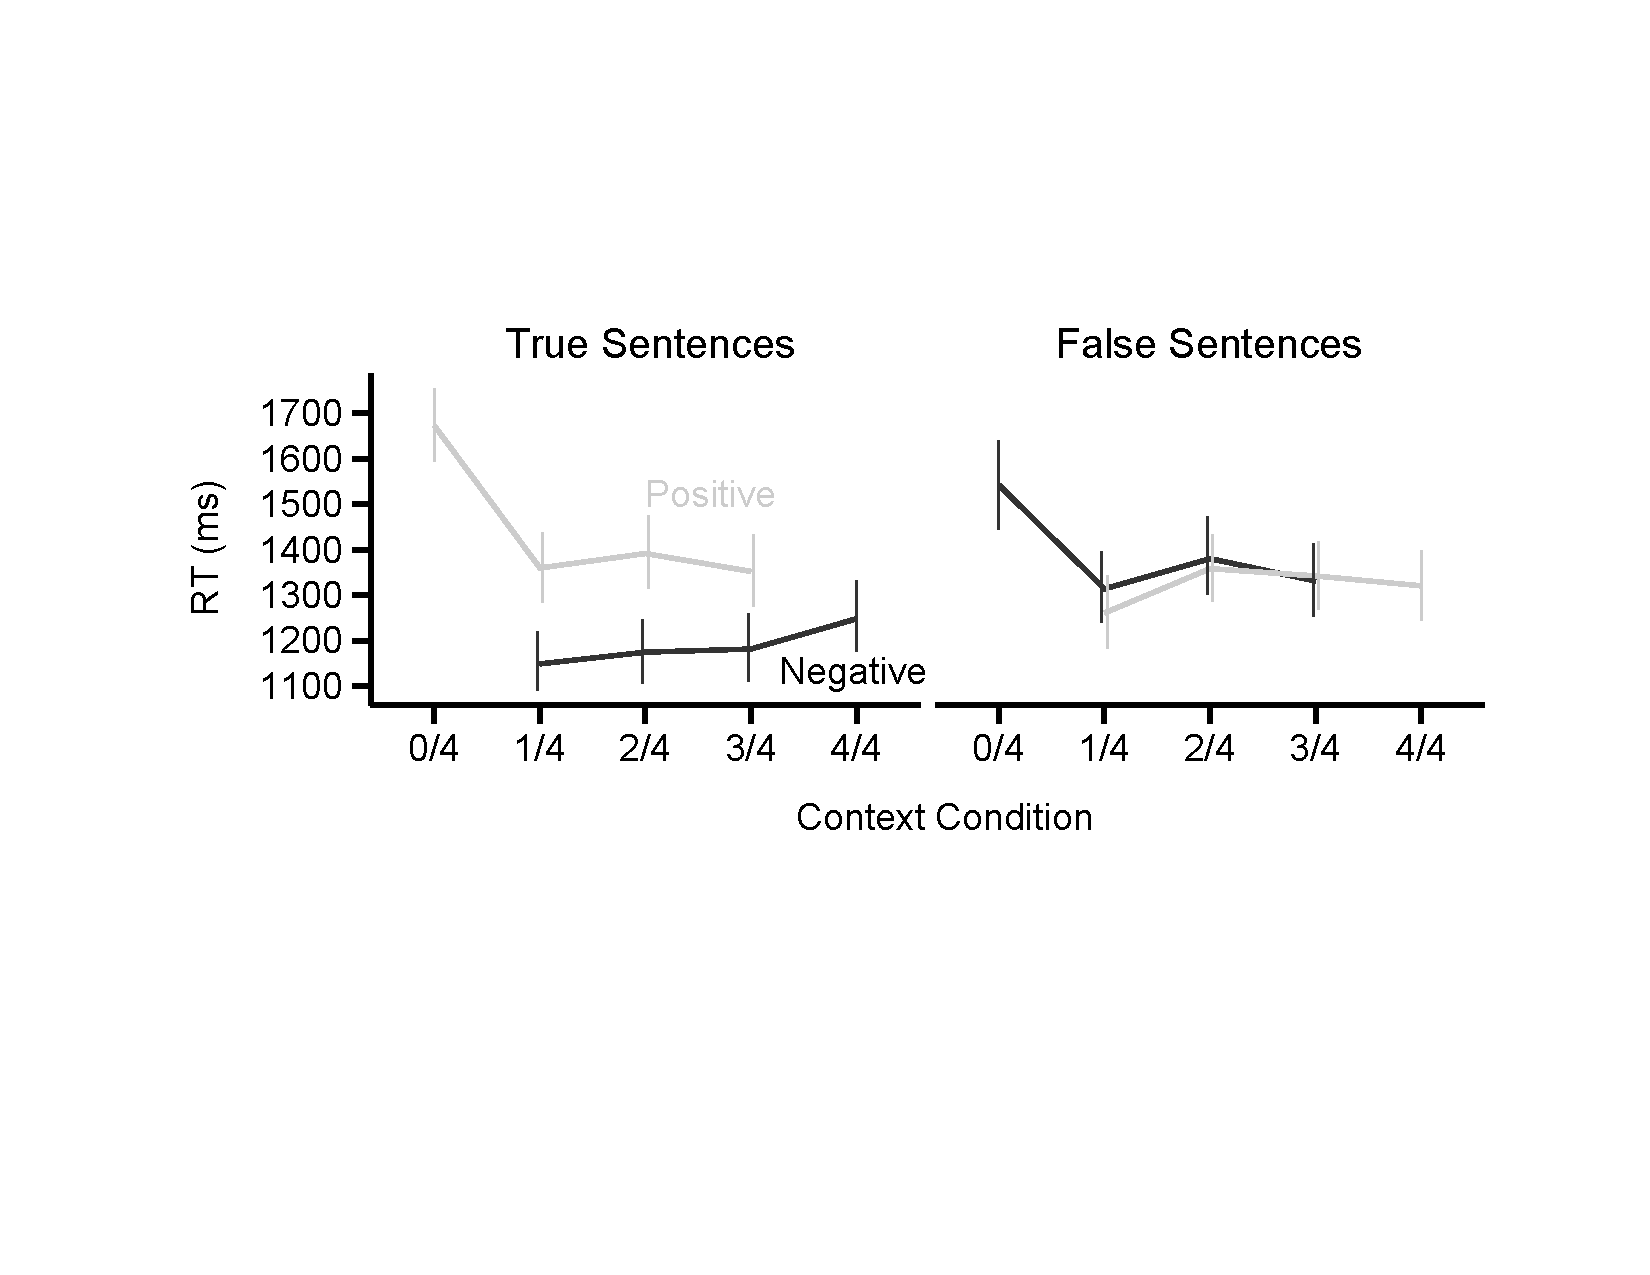
\includegraphics[width=4.5in]{figures/rts.pdf}
\caption{\label{fig:e2line} Reaction times for each trial type across different conditions. Responses to true sentences are shown on the left, and false sentences are shown on the right.  Negative sentences are shown in grey, and positive sentences in black.  The context condition is notated by a fraction representing the number of characters in the context who held target items. Error bars show 95\% confidence intervals computed by non-parametric bootstrapping.  }
\end{center} 
\end{figure}

Participants were fastest to respond to true positive sentences, and slowest to respond to true negative sentences.  Responses to true negative sentences showed the most pronounced effect of context, with reaction times in response to negative sentences decreasing as the proportion of target items in the context increased.  Responses to false positive sentences showed a similar but less pronounced effect of context, and responses to true positive and false negative sentences showed a slight but reversed effect of context, with increased reaction times as the proportion of target items in the context increased.  

To evaluate the reliability of these patterns, we fit a linear mixed-effects model to reaction times in response to sentences.  We examined the interaction between sentence type (i.e. positive or negative sentences), truth value (i.e. true or false sentences), and context condition on reaction times.\footnote{All mixed-effects models were fit using the lme4 package version 1.1-7 in R version 3.1.2.  The model specification was as follows: \texttt{RT $\sim$ sentence~$\times$~truth~$\times$~context + (sentence~\textbar~subject) +  (sentence~\textbar~item)}.  Significance was calculated using the standard normal approximation to the $t$ distribution \cite{barr2013}. Data and analysis code can be found at FILL THIS IN LATER.}  Results of this model showed an interaction between sentence type and truth value, such that true positive sentences elicited the fastest responses and true negative sentences elicited the slowest responses ($\beta= 895$, $p< .001$).  The model showed a significant negative linear effect of context, with reactions times decreasing as the proportion of characters with target items increased ($\beta= -59$, $p< .001$), but a significant three-way interaction between sentence type, truth value, and context indicates that this is driven primarily by responses to true negative sentences $\beta= -209$, $p< .001$), with true positive and false negative sentences showing a smaller positive linear effect of context.  

\begin{table}[t]
\caption{Coefficient estimates from a mixed-effects model predicting listeners' reaction times in response to sentences in different context conditions.}
\begin{center}
\small\addtolength{\tabcolsep}{-5pt}
\begin{tabular}{rrrr}
  \hline
 & Coefficient & Std. err. & t value \\ 
  \hline
(Intercept) & 1541 & 45 & 34.20 \\ 
  Sentence (Negative) & -282 & 50 & -5.63  \\ 
  Truth value (True) & -461 & 50 & -9.29 \\
  Context & -59 & 11 & -5.44 \\ 
  Sentence$\times$Truth value & 895 & 71 & 12.65 \\
  Sentence$\times$Context & 78 & 15 & 5.05 \\
  Truth value$\times$Context & 92 & 15 & 5.97 \\
  Sentence$\times$Truth value$\times$Context & -209 & 22 & -9.52 \\
   \hline
\end{tabular}
\vspace{-1.5cm}
\end{center}
\end{table}

\subsection{Speaker Condition}

\begin{figure}[t]
\begin{center} 
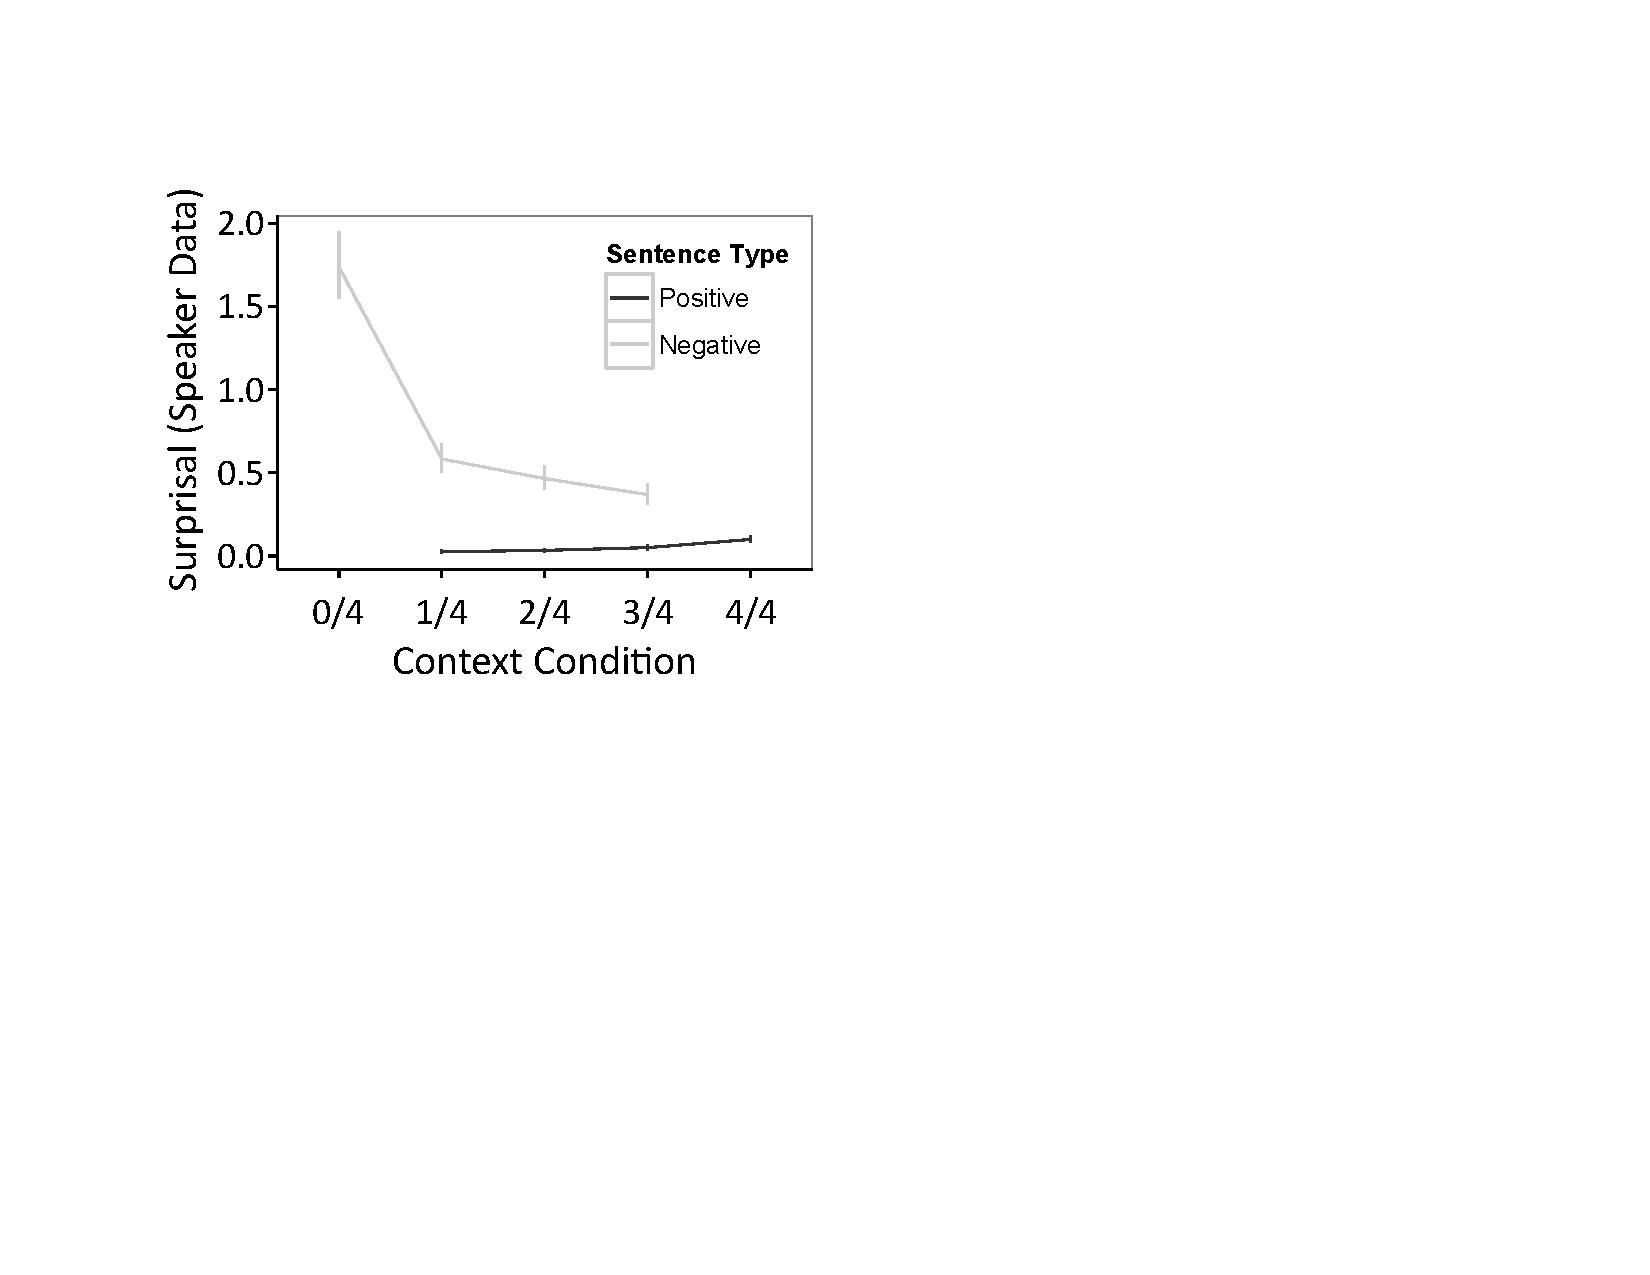
\includegraphics[width=3in]{figures/surprisals.pdf}
\caption{\label{fig:e2line} \textcolor{blue}{FIXME} Surprisal for true positive and true negative sentences across different conditions. On the left is a plot of surprisal computed using data from the speaker condition of the experiments.  Negative sentences are shown in grey, and positive sentences in black.  The context condition is notated by a fraction representing the number of characters in the context who held target items. Error bars show 95\% confidence intervals computed by non-parametric bootstrapping.  }
\end{center} 
\end{figure}

We hypothesized that the processing cost of negation could be explained by the Gricean intuition that listeners expect speakers to produce informative utterances.  To link pragmatic expectations to reaction time, we assume that reaction time is proportional to \emph{surprisal}. Surprisal is an information-theoretic measure of the amount of information carried by an event (in this case, an utterance in some context) based on its probability. Surprisal has been used effectively to predict reaction times from probabilistic models \cite{levy2008}; here, we used the probability of participants in the speaker condition producing a true positive or a true negative utterance in different contexts to calculate pragmatic surprisal.

Surprisal was much higher for negative sentences compared to positive sentences across all context conditions.  Negative sentences in the $\frac{0}{4}$ condition had the highest surprisal, and positive sentences in the $\frac{1}{4}$ condition had the lowest surprisal.  For negative sentences, surprisal decreased as the number of characters with target items increased, and for positive sentences surprisal increased as the number of characters with target items increased.  

%More here
To test the hypothesis that sentence processing is related to listeners' expectations about what a speaker will say, we plotted the mean reaction time in response to true positive and negative utterances in each condition against the surprisal for the same utterances.  There was a significant posiitve correlation between surprisal and reaction time for true negative sentences, $r=.97$, $p<.001$, supporting our prediction that the effects of context on reaction time were driven by differences in how speakers' described the stimuli.  


\begin{figure}[t]
\begin{center} 
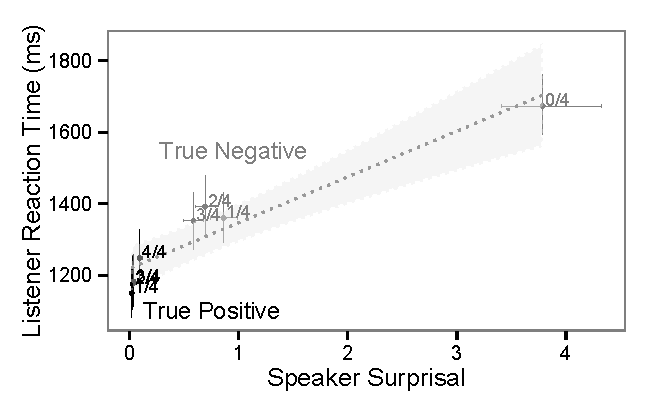
\includegraphics[width=4in]{figures/production_rts.pdf}
\caption{\label{fig:scatter} ... }
\end{center} 
\end{figure}

\section{General Discussion}

We found that participants were faster to respond to and more likely to produce negative sentences when a greater proportion of characters in the context possessed the negated item.  This was consistent with our hypothesis that the processing cost of negation is due to general pragmatic principles about how listeners expect speakers to behave.  We suggested a Gricean account of these data: The processing cost of negation is related to the degree to which it violates expectations about communication in context. In our studies, by changing the proportion of people in the context who held a target item, we systematically manipulated participants' contextual expectations.  We found a parametric relationship between the strength of the context and reaction times, and this relationship was well fit by participants' descriptions of the stimuli in different contexts.

Previous work on sentence processing has suggested that processing negation is fundamentally difficult, perhaps due to the processing cost of negating a proposition (e.g.\ \citeNP{hclark1972}) or the cost of suppressing an affirmative representation (e.g.\ \citeNP{kaup2003}).  Our work here suggests that the difficulty of negation may not be unique to negation at all; instead, general pragmatic mechanisms could be driving this effect.  Due to the specific pragmatics of negation, negative sentences presented without context are uninformative and are thus unlikely to be produced, leading to increased surprisal and slower processing times.  In conversation, however, negative sentences are often produced when some expectation has been violated, decreasing surprisal and processing time.  

What is the mechanism by which context influences the probability of producing a negative utterance?  One possibility is that negative sentences are more informative in contexts that set up a strong expectation that is violated. If the processing cost of negation is pragmatic, then more informative negative sentences should elicit smaller reaction times.  Recent modeling work quantifies pragmatic reasoning in simple experimental contexts \cite{frank2012,goodman2013}. The assumption underlying this work is that speakers are informative---they will produce utterances that will pick out smaller subsets of the context, leaving as little ambiguity as possible for the listener.  This prediction is reflected in our results: True negative utterances were more informative in contexts where more people possessed the negated item, and these contexts elicited the highest rate of negation from speakers and the fastest reaction times from listeners. Another possibility is that a speaker's utterance are influenced by the ``Question Under Discussion'' (QUD; \citeA{roberts1996}). In our experiment, articipants were slowest to respond to trials where none of the characters possessed the objects that were mentioned in the sentence; e.g. ``Bob has/has no apples'' in response to a context where none of the boys are holding anything.  In addition to being uninformative, these sentences might have incurred additional processing costs due to the mention of an unexpected topic.  

%Our analyses focused on true sentences, because of our interest in exploring participants' expectations about how an informative speaker should behave.  Due to the nature of our task, participants in the listener condition likely expected some of the sentences to be false, but it is not clear what constitutes an ``informative'' false sentence.  Our listener data replicate an interaction between sentence type and truth value that is seen frequently in literature on sentence verification tasks \cite{hclark1972}, with false positive sentences showing a similar pattern as true negative sentences.  


Although our specific focus was to understand the processing of negative sentences, this work has implications for sentence processing more generally.  Debates about the effects of pragmatics on linguistic processing exist in other domains, such as the processing of scalar implicatures, \citeNP{huang2009, huang2011, grodner2010}.  For example, \citeA{tomlinson2013} present mouse-tracking data to argue that that processing scalar implicatures is cognitively demanding. Their data, however, are also consistent with our hypothesis that listeners' responses to different sentences are influenced by pragmatic surprisal; in their experiments, participants showed the same mouse-tracking patterns in response to underinformative scalar implicatures as well as underinformative negative utterances.  We believe that formal models of pragmatics can provide insight into these debates and, more generally, into the role that pragmatic context plays in linguistic processing. 
 



\bibliographystyle{apacite}

\setlength{\bibleftmargin}{.125in}
\setlength{\bibindent}{-\bibleftmargin}

\bibliography{negation}

\end{document}


%Maybe move some of this to the GD
%What is the mechanism by which context influences the processing of negation?  We propose that negative sentences are more informative in contexts that set up a strong expectation that is violated. If the processing cost of negation is pragmatic, then more informative negative sentences should elicit smaller reaction times. How should we quantify informativeness in context? Recent modeling work quantifies pragmatic reasoning in simple experimental contexts \cite{frank2012,goodman2013}. The assumption underlying this work is that speakers are informative---they will produce utterances that will pick out smaller subsets of the context, leaving as little ambiguity as possible for the listener.  We use this definition of informativeness to provide a quantitative interpretation of our hypothesis.

%MOVE THIS:
%To link pragmatic expectations to reaction time, we assume that reaction time is proportional to \emph{surprisal}. Surprisal is an information-theoretic measure of the amount of information carried by an event (in this case, an utterance in some context) based on its probability. Surprisal has been used effectively to predict reaction times from probabilistic models \cite{levy2008}; in this work, we directly measure the probability of an utterance occurring by eliciting descriptions of our stimuli from our participants.